% Chapter Template

\chapter{Phase 1 - Investigation} % Main chapter title

\label{Chapter4} % Change X to a consecutive number; for referencing this chapter elsewhere, use \ref{ChapterX}

%----------------------------------------------------------------------------------------
%	SECTION 1
%----------------------------------------------------------------------------------------
The goal of the Investigation phase is to gain a deeper understanding of the differences between Chinese and western websites. Then using this information we will decide on what features we want to analyse and what usability metrics we want to use for this.
\section{Method}
Firstly, several Chinese websites and their western counterparts were identified and the main differences that had to do with the project scope were analyzed. Secondly, a conclusion where what design patterns that will to be tested was selected. What metrics to use to measure these design differences were also decided.

\section{Results}
\section{Chinese vs Western websites comparison}
Chinese websites are clearly very different in design compared to their western counterparts. The differences are more that just the look and feel of the sites but also the UX design of the sites are very different. We will look at some of Chinas biggest and most popular websites and in some cases compare them to the English counterparts. 

\subsection{QQ}
QQ is one of the top most visited website in China (see fig \ref{fig:QQ.com}). \cite{top_sites_china} \cite{top_sites_alexa} QQ like many other Chinese websites does not focus on one thing but has many different functions. Part of the functionality that QQ offer is: instant messaging, online social games, music, shopping, microblogging, news, movies, group and voice chat software etc. Going to the main homepage (QQ.com) you will be greeted by their news page. As we can see this page is quite information dense. If we count all the clickable elements without hovering over anything on a standard computer screen we get about 147 clickable elements . If we compare this to BBC's homepage \cite{bbc} which is considered fairly information dense by western standards. (source??) It has 48 clickable elements on its homepage. This means that QQ has over 3 times as many clickable elements as BBC.


\begin{figure}[h]
\centering
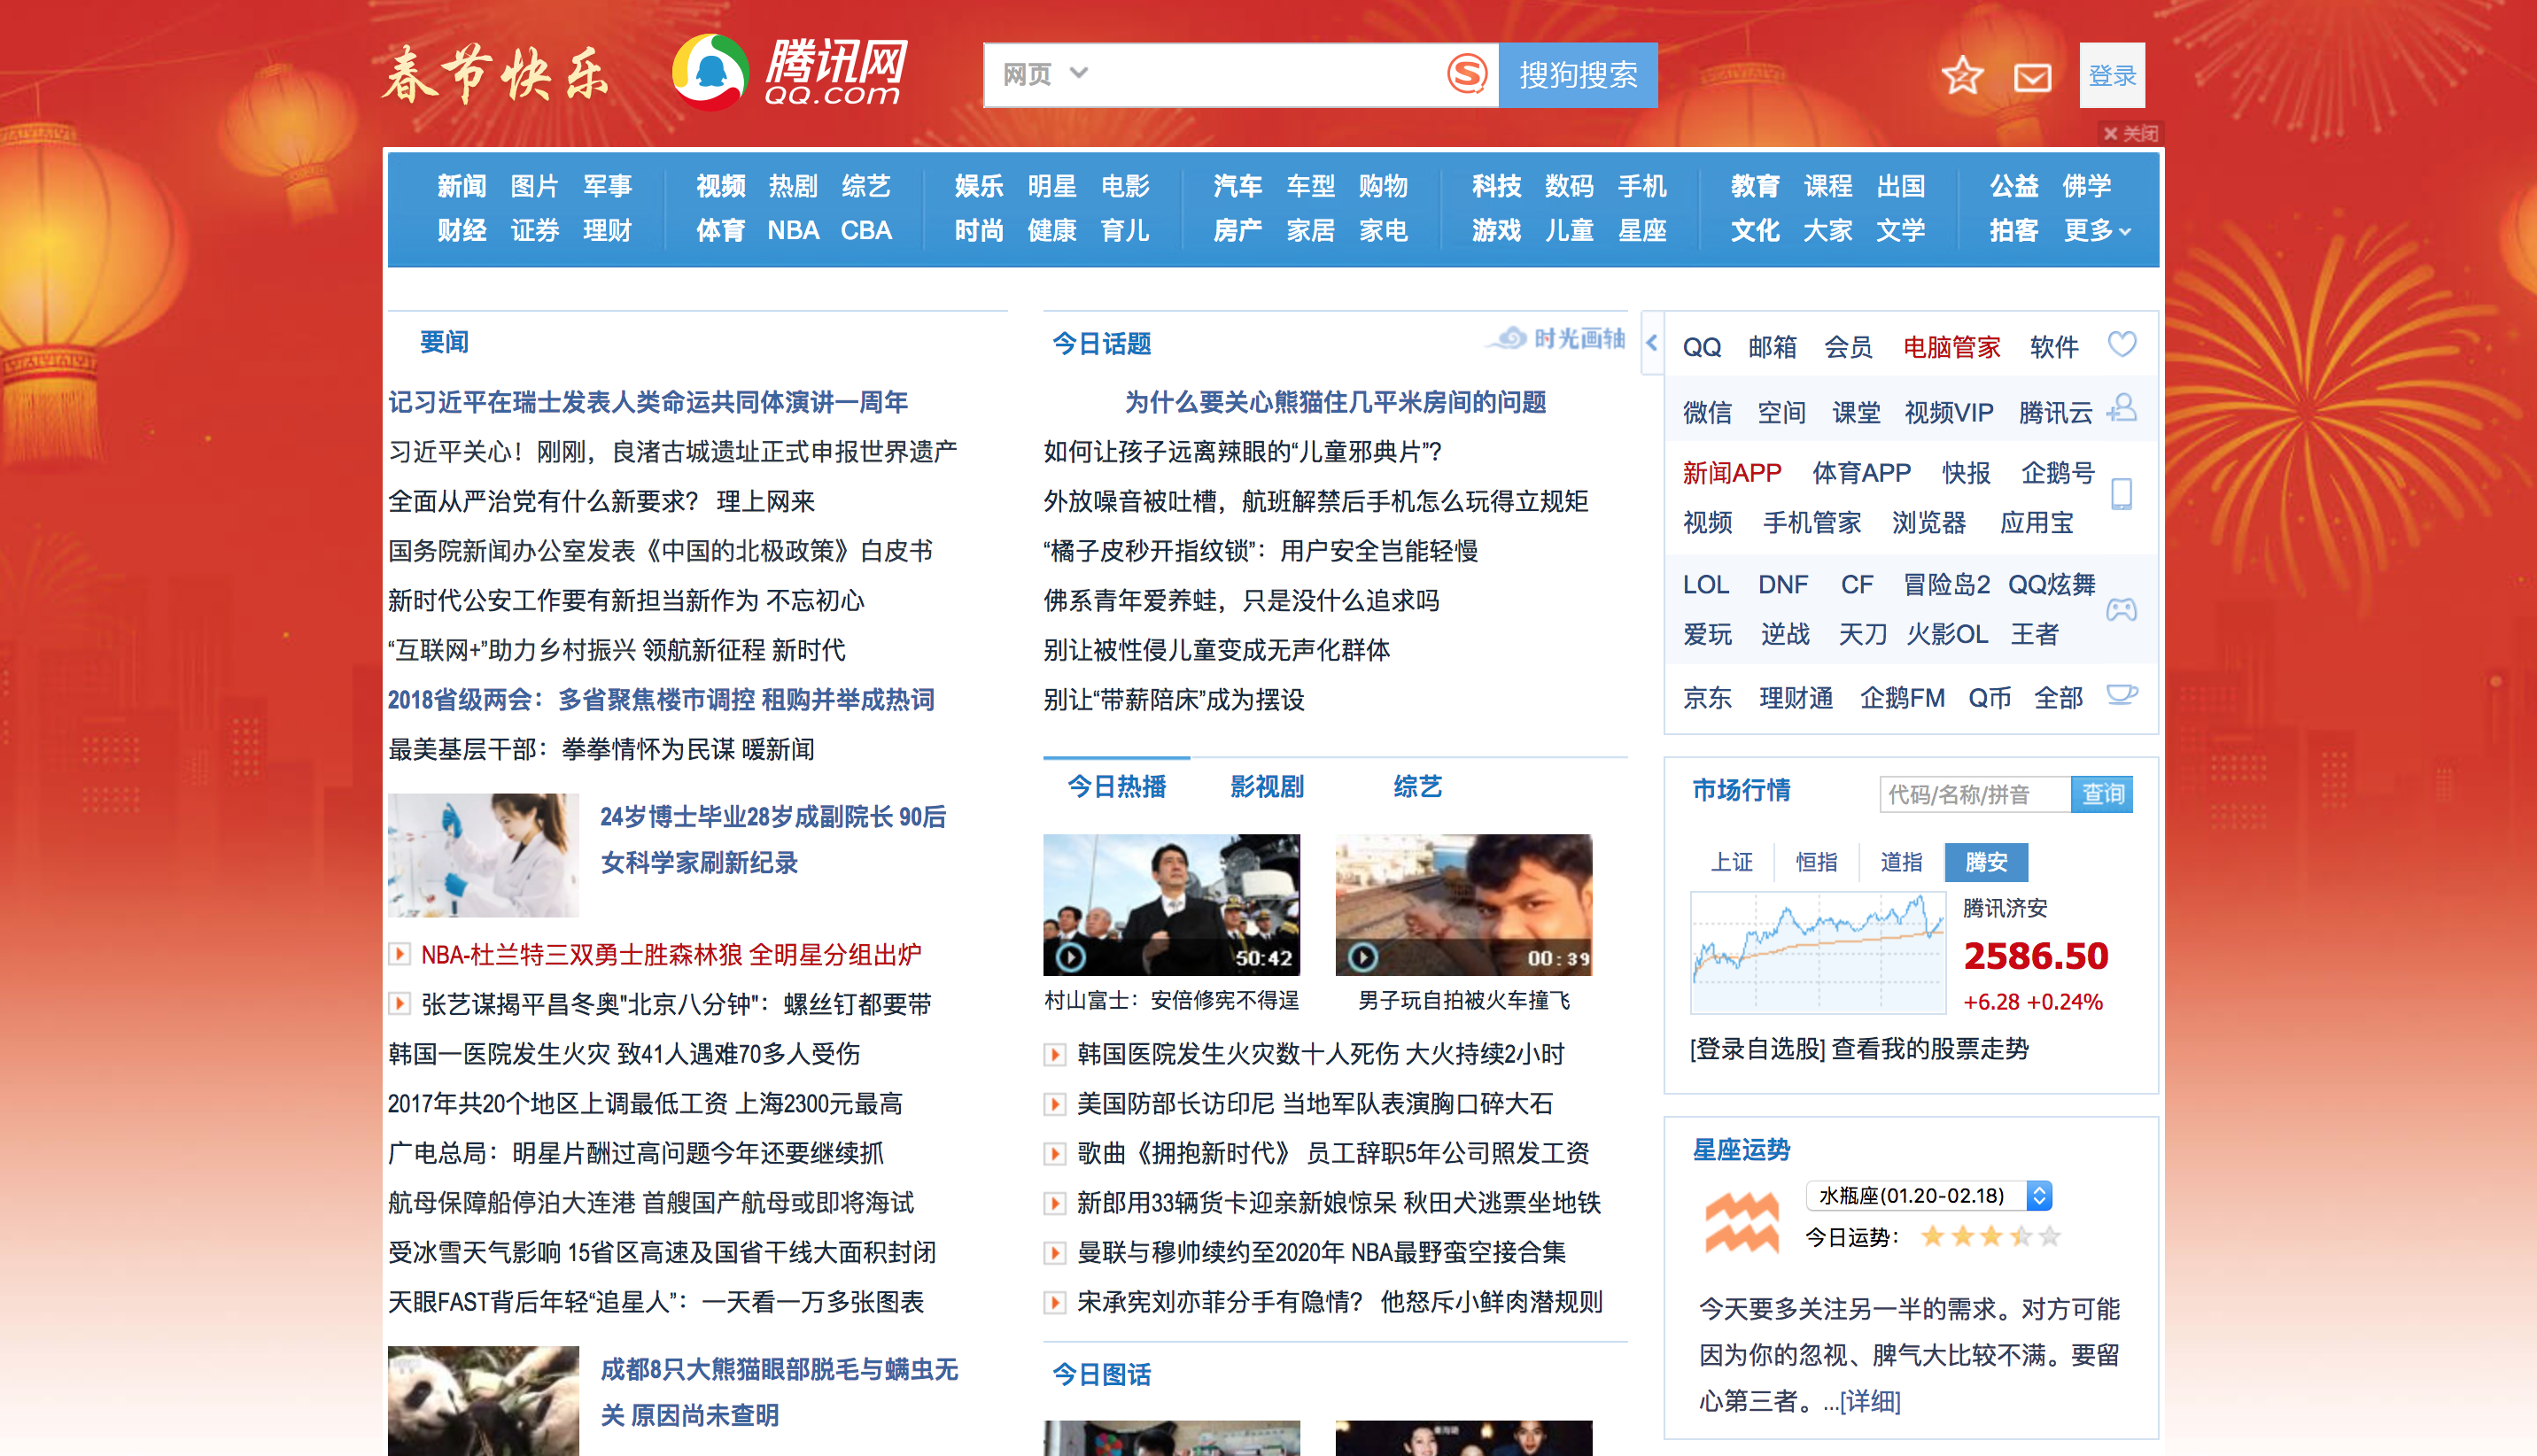
\includegraphics[width=100mm]{Images/QQ.png}
\decoRule
\caption[QQ.com]{QQ's homepage which provide which is mostly used for news.}
\label{fig:QQ.com}
\end{figure}

One element that is quite common on Chinese websites that we can see in QQ as well is it's menu bar (see fig \ref{fig:QQ_menubar}). This menu bar has two rows with a total of 40 options. This type of menu bar is quite common and can be seen at many other Chinese sites.


\begin{figure}[h]
\centering
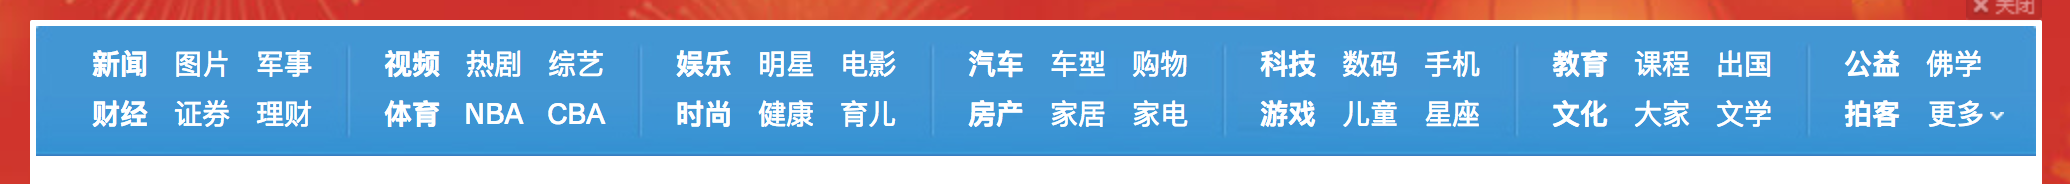
\includegraphics[width=100mm]{Images/QQ_menubar.png}
\decoRule
\caption[QQ's Menu bar]{A close-up of the menu bar used at QQ.}
\label{fig:QQ_menubar}
\end{figure}

\subsection{Taobao and Ebay}
Taobao is one of the biggest websites in the world. Taobao is similar to the American Ebay in terms of what the website provide. They both are online shopping websites where you can almost everything you need. The design and user-experience focus on the sites are quite different. Ebay has a very sleek design with darker colors and only 20 clickable elements (see fig:\ref{fig:ebay}). Ebay also have expanding menu bar that contains about 6-10 clickable elements (see fig:\ref{fig:ebay_menu}).

\begin{figure}[h]
\centering
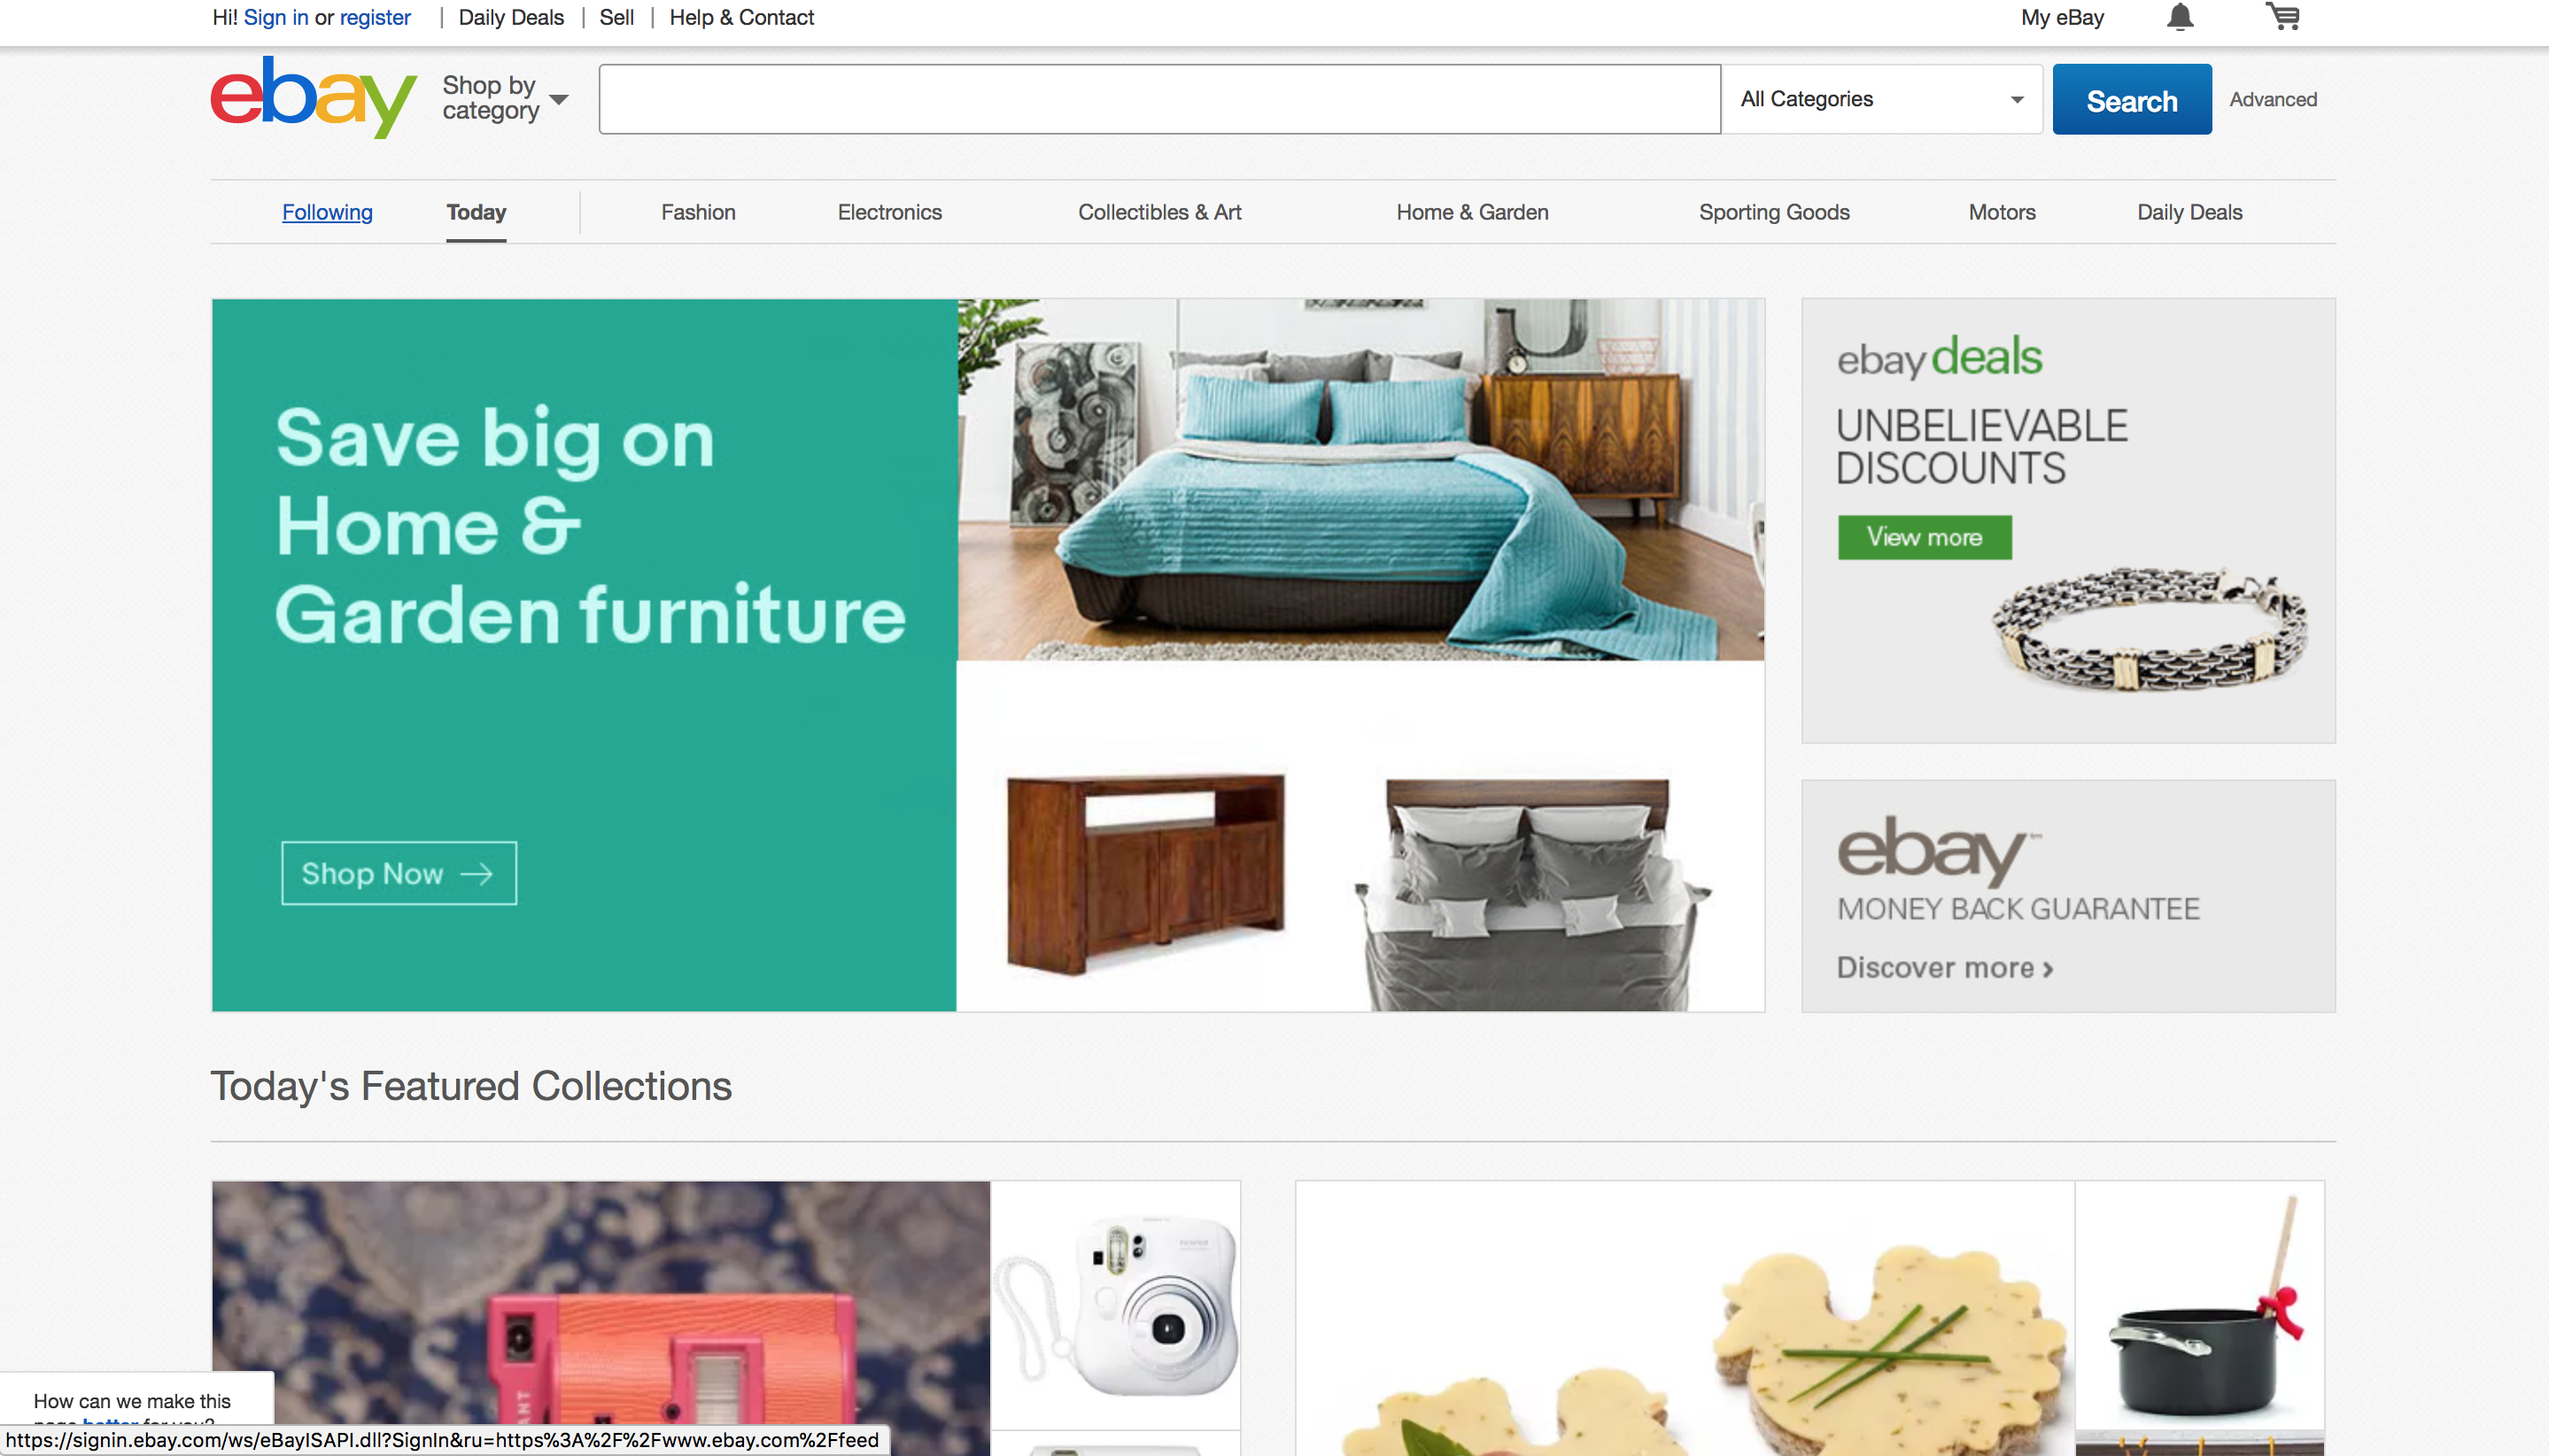
\includegraphics[width=100mm]{Images/ebay.png}
\decoRule
\caption[ebay]{Ebay a popular American online shopping site}
\label{fig:ebay}
\end{figure}

\begin{figure}[h]
\centering
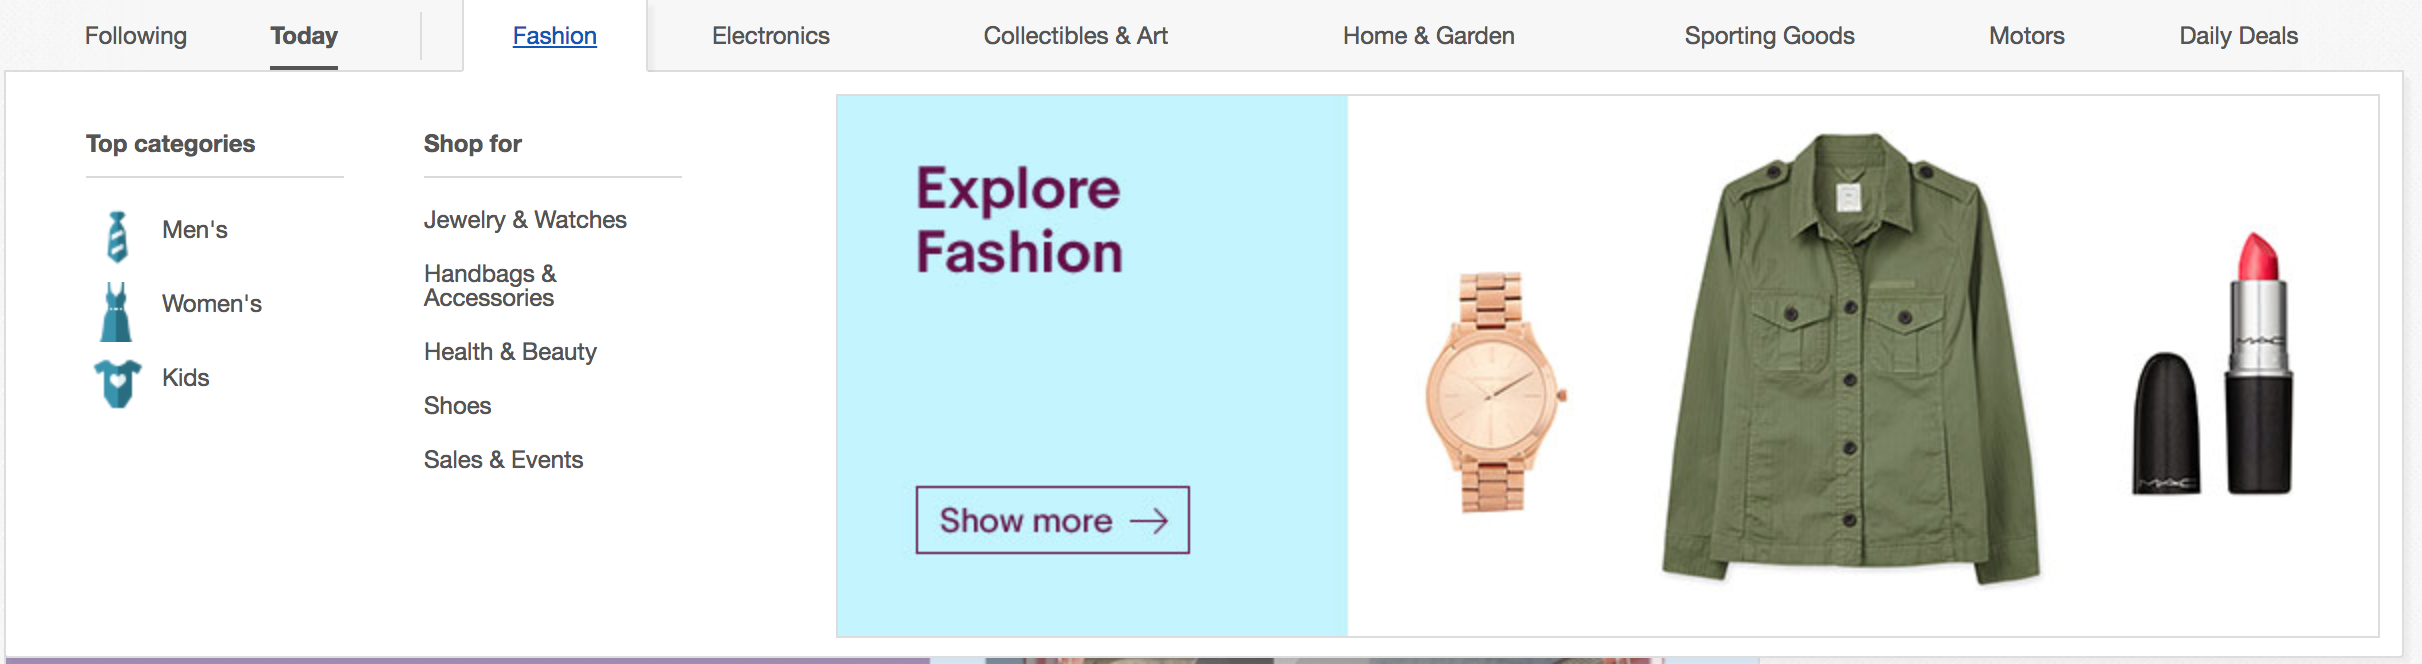
\includegraphics[width=100mm]{Images/ebay_menu.png}
\decoRule
\caption[Ebay's menu bar]{Expanding the menu on Ebay.}
\label{fig:ebay_menu}
\end{figure}

If we look at the Chinese version Taobao we once again can clearly tell the difference in information density (see fig:\ref{fig:taobao}). The main page has about 49 clickable elements. And the menu items on the right hand side can expand and show between 55-80 clickable links and elements (see fig:\ref{fig:taobao_menu}). That is about 8 times more clickable elements compared to Ebay. Another thing we can see that is very with Taobao is the strong colors, Taobao frequently use very strong red, purple, orange and blue. Ebay keeps more to gray and let their products provide the stronger colors to make you focus on them. 

\begin{figure}[h]
\centering
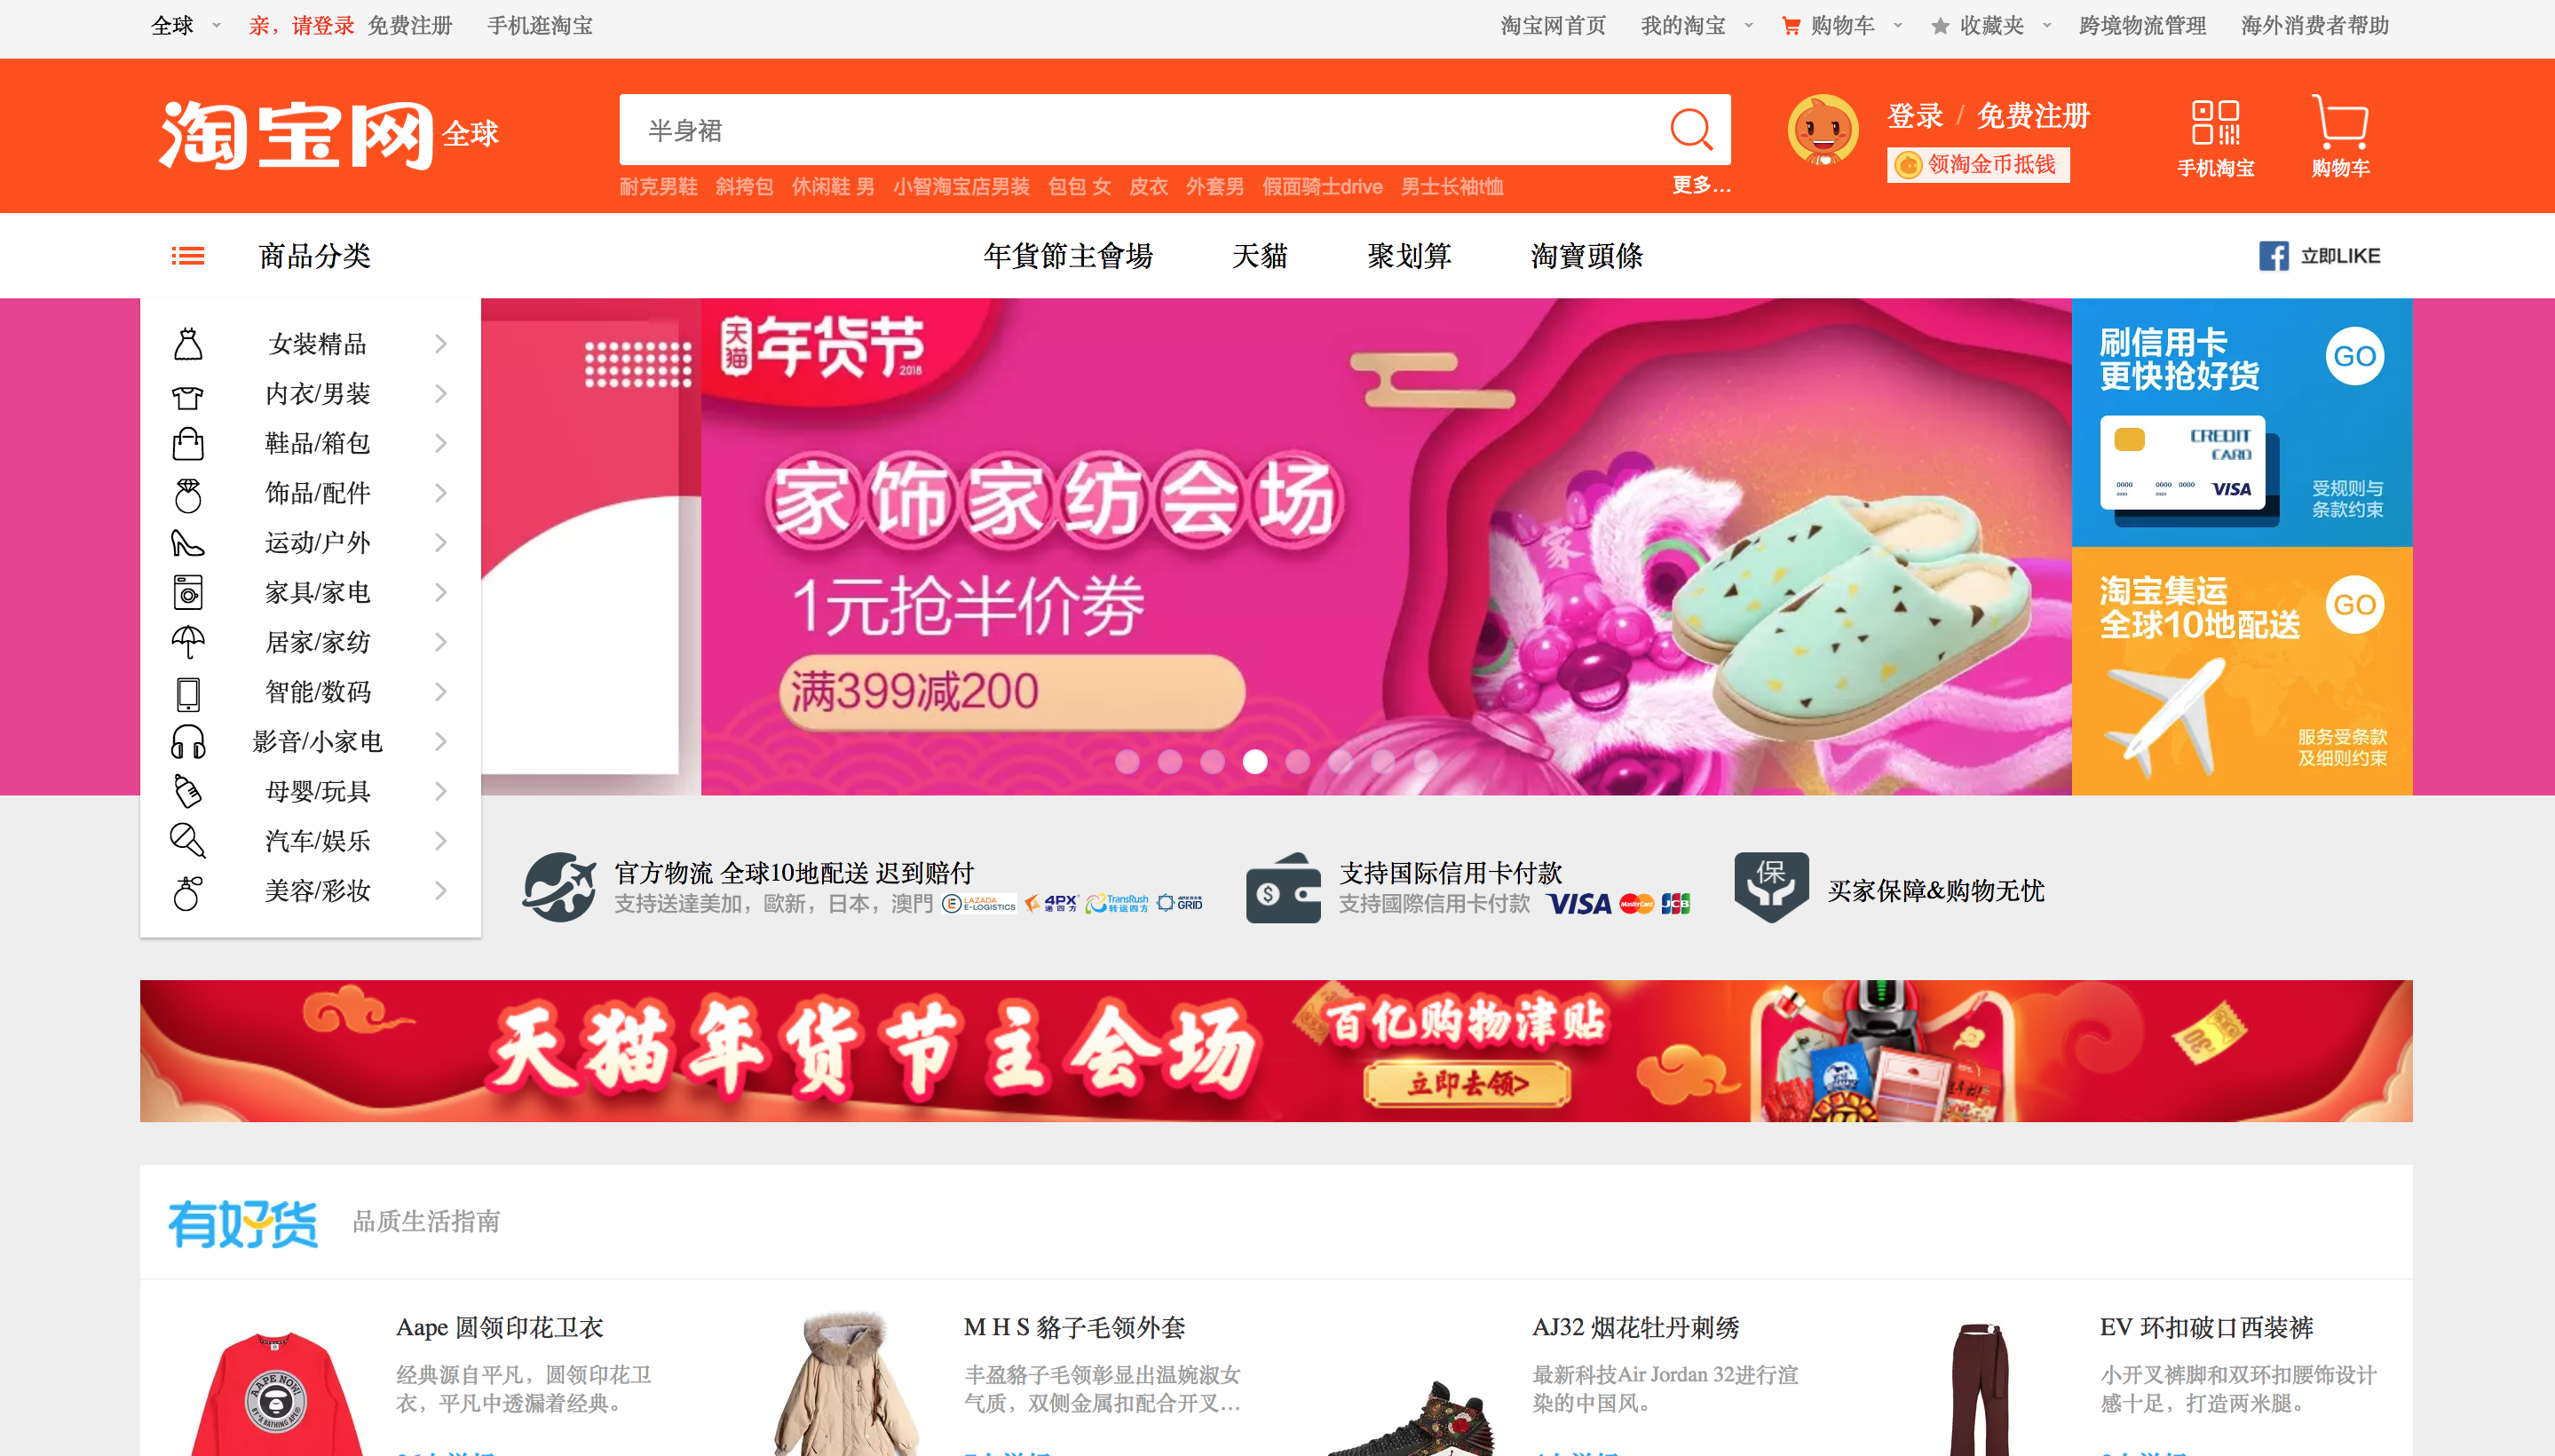
\includegraphics[width=100mm]{Images/Taobao}
\decoRule
\caption[Taobao]{Taobao a popular Chinese online shopping site}
\label{fig:taobao}
\end{figure}

\begin{figure}[h]
\centering
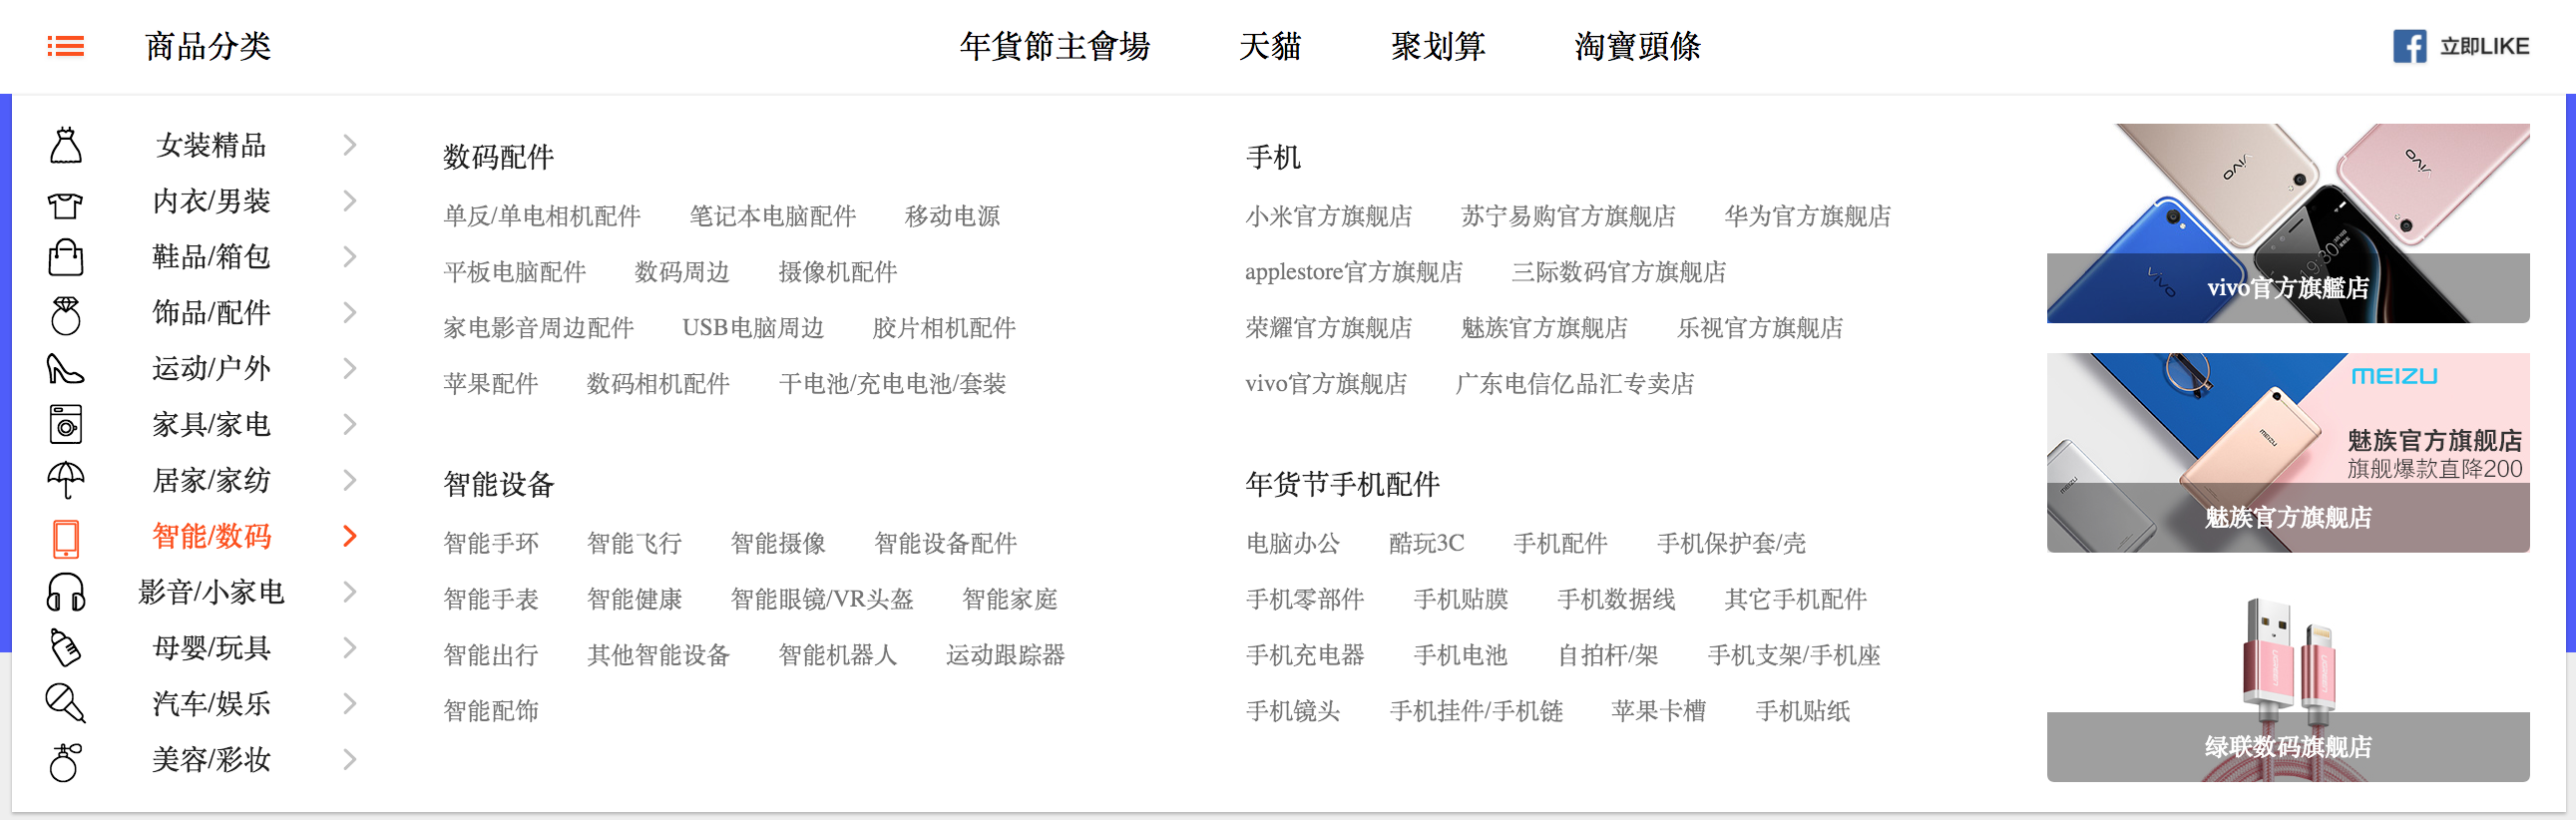
\includegraphics[width=100mm]{Images/Taobao_menu}
\decoRule
\caption[Taobao' menu bar]{Expanding the menu on Taobao.}
\label{fig:taobao_menu}
\end{figure}

\subsection{Analyses of Ctrip}
Many Chinese web sites change quite a lot when changing language. Ctrip is one of these sites. Ctrip is a very common travel site in China which allows you to book hotels, flights, car rental etc. When you select to translate this site to English it does not only translate the site but the whole layout and design of the website change as well (see  fig: \ref{fig:ctrip_chinese} for Chinese version and fig: \ref{fig:ctrip_english} for English version). Except for the brand and name of the website you can barely tell that it is the same website.
\begin{figure}[h]
\centering
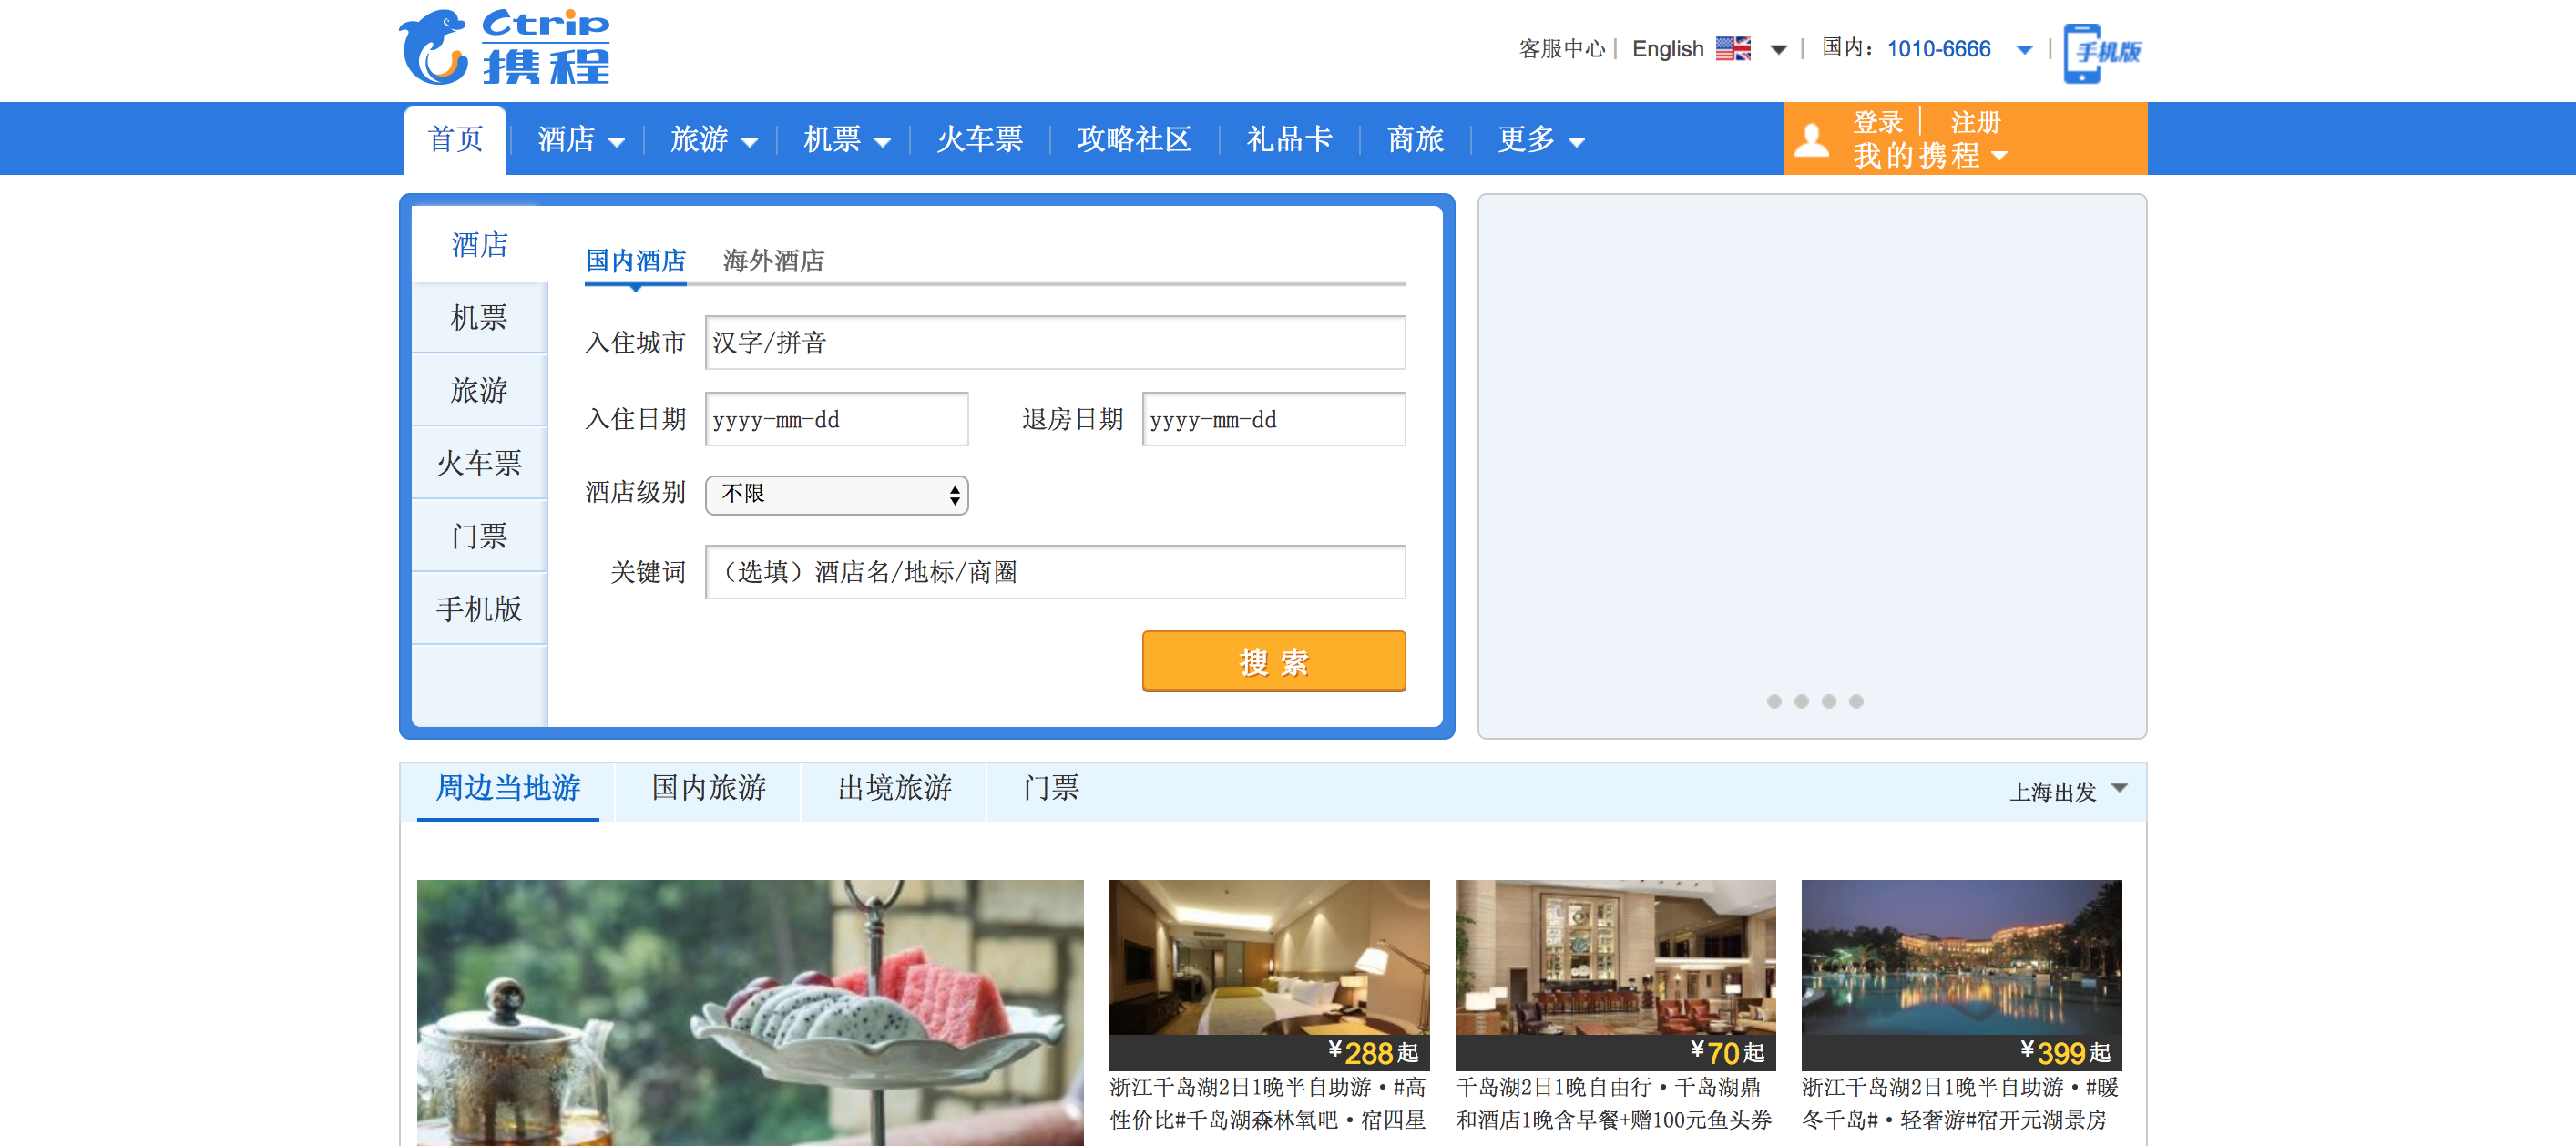
\includegraphics[width=100mm]{Images/ctrip_chinese1}
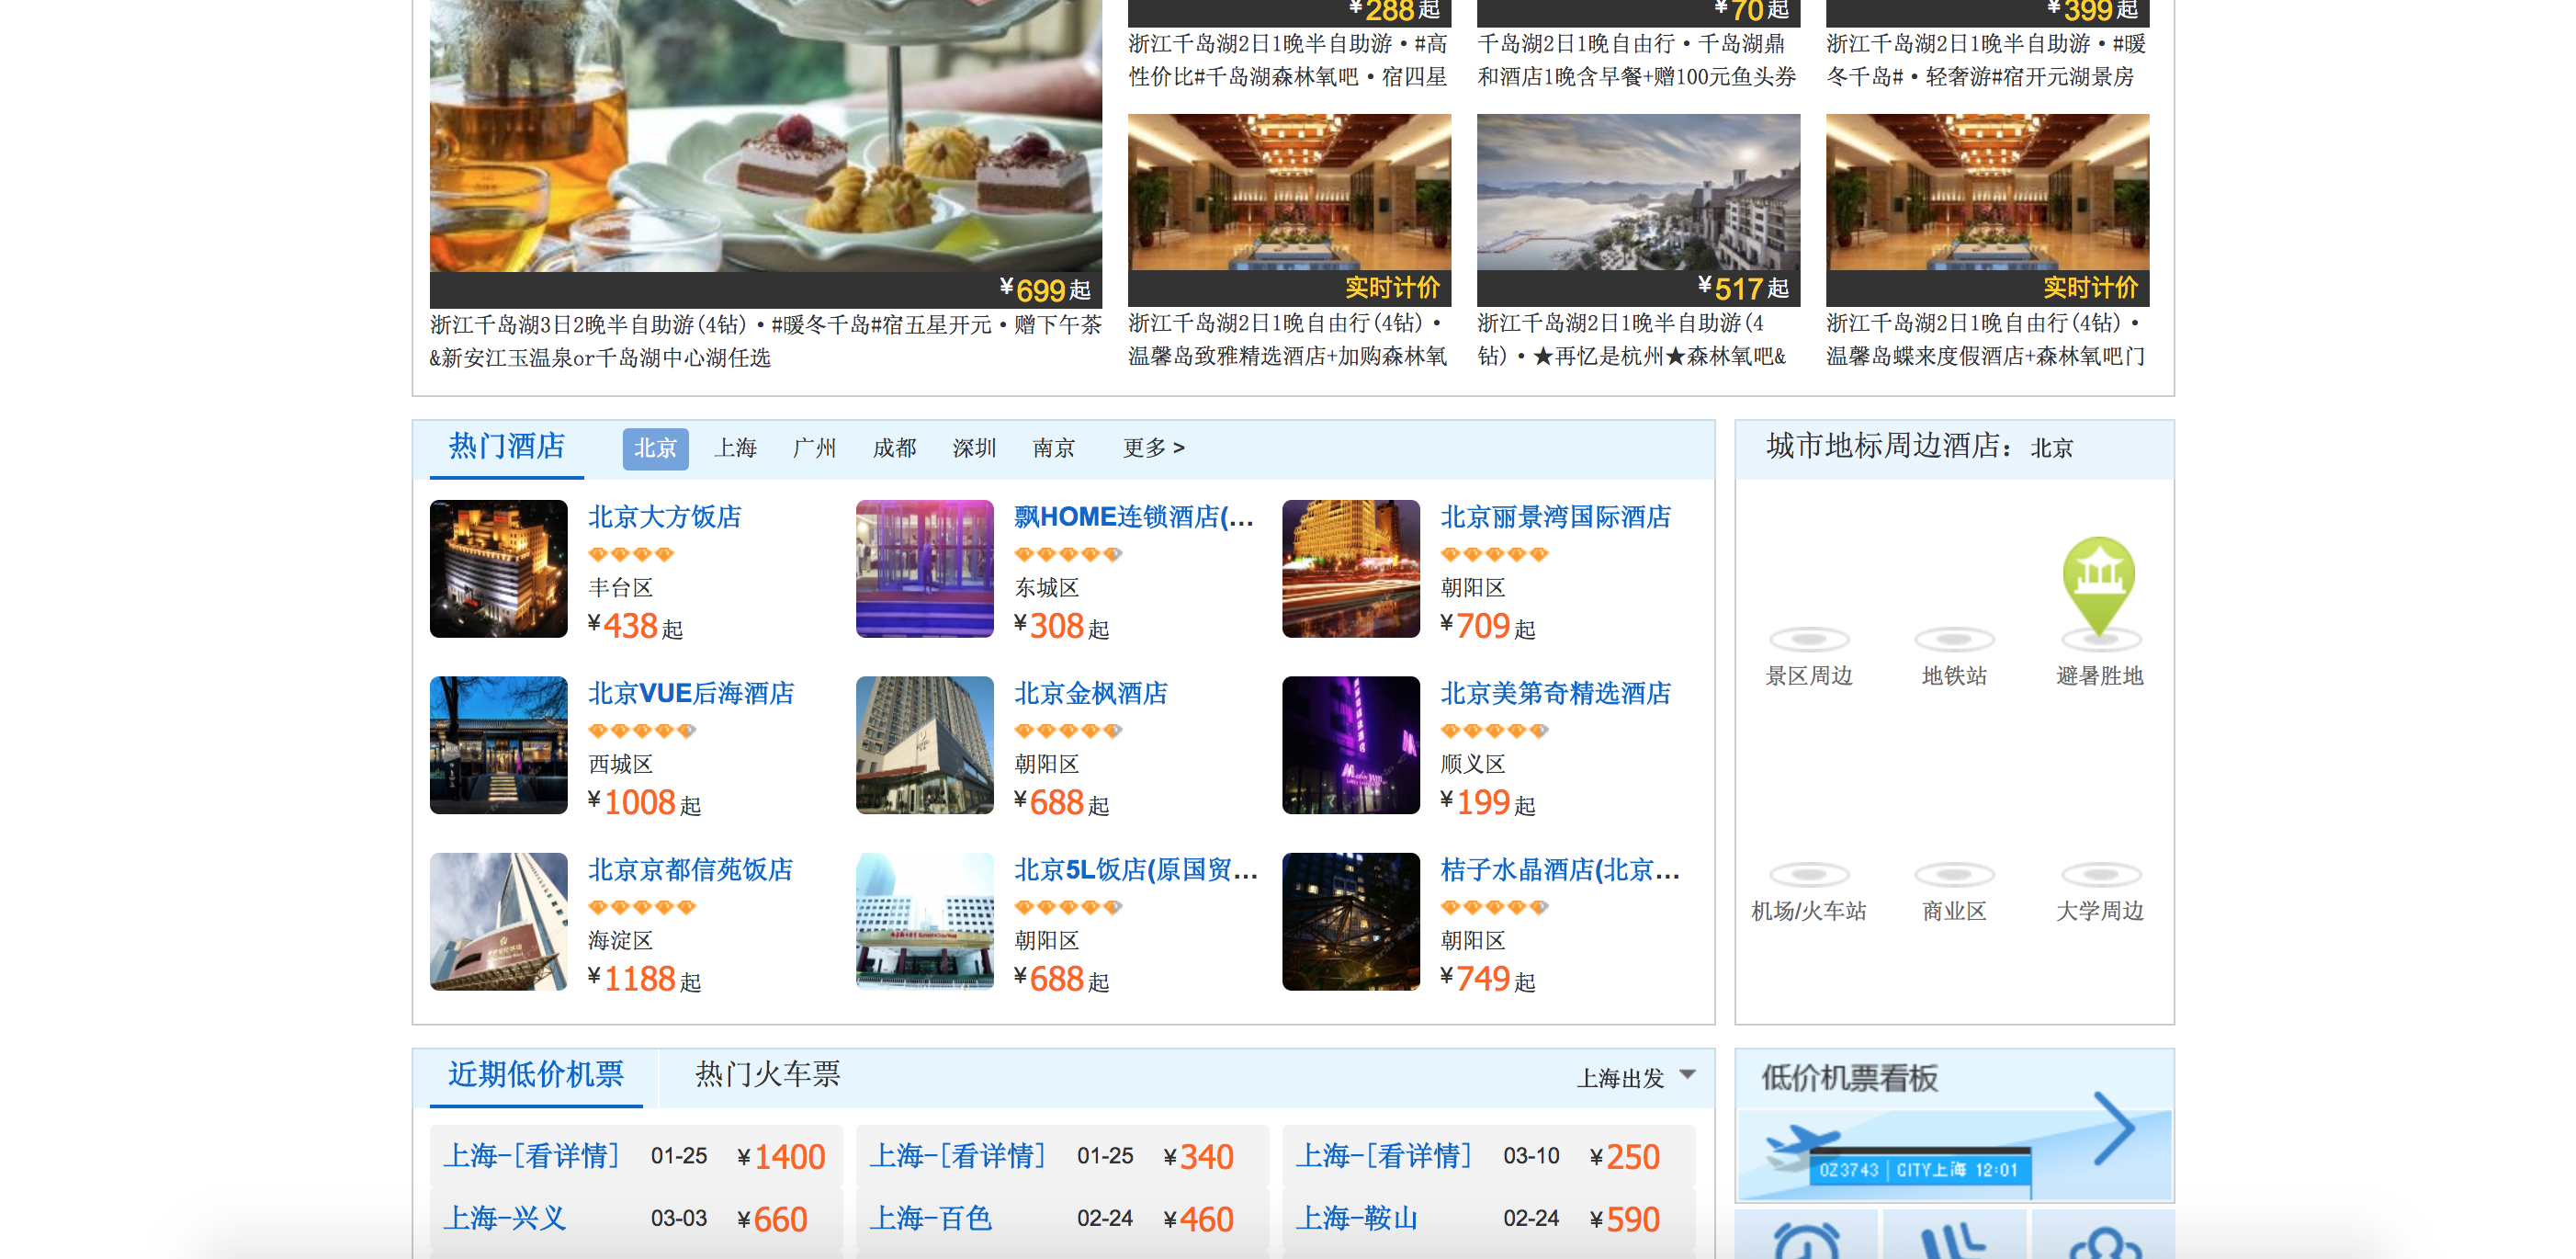
\includegraphics[width=100mm]{Images/ctrip_chinese2}
\decoRule
\caption[Chinese version of Ctrip]{The Chinese version of the travel website Ctrip.}
\label{fig:ctrip_chinese}
\end{figure}

\begin{figure}[h]
\centering
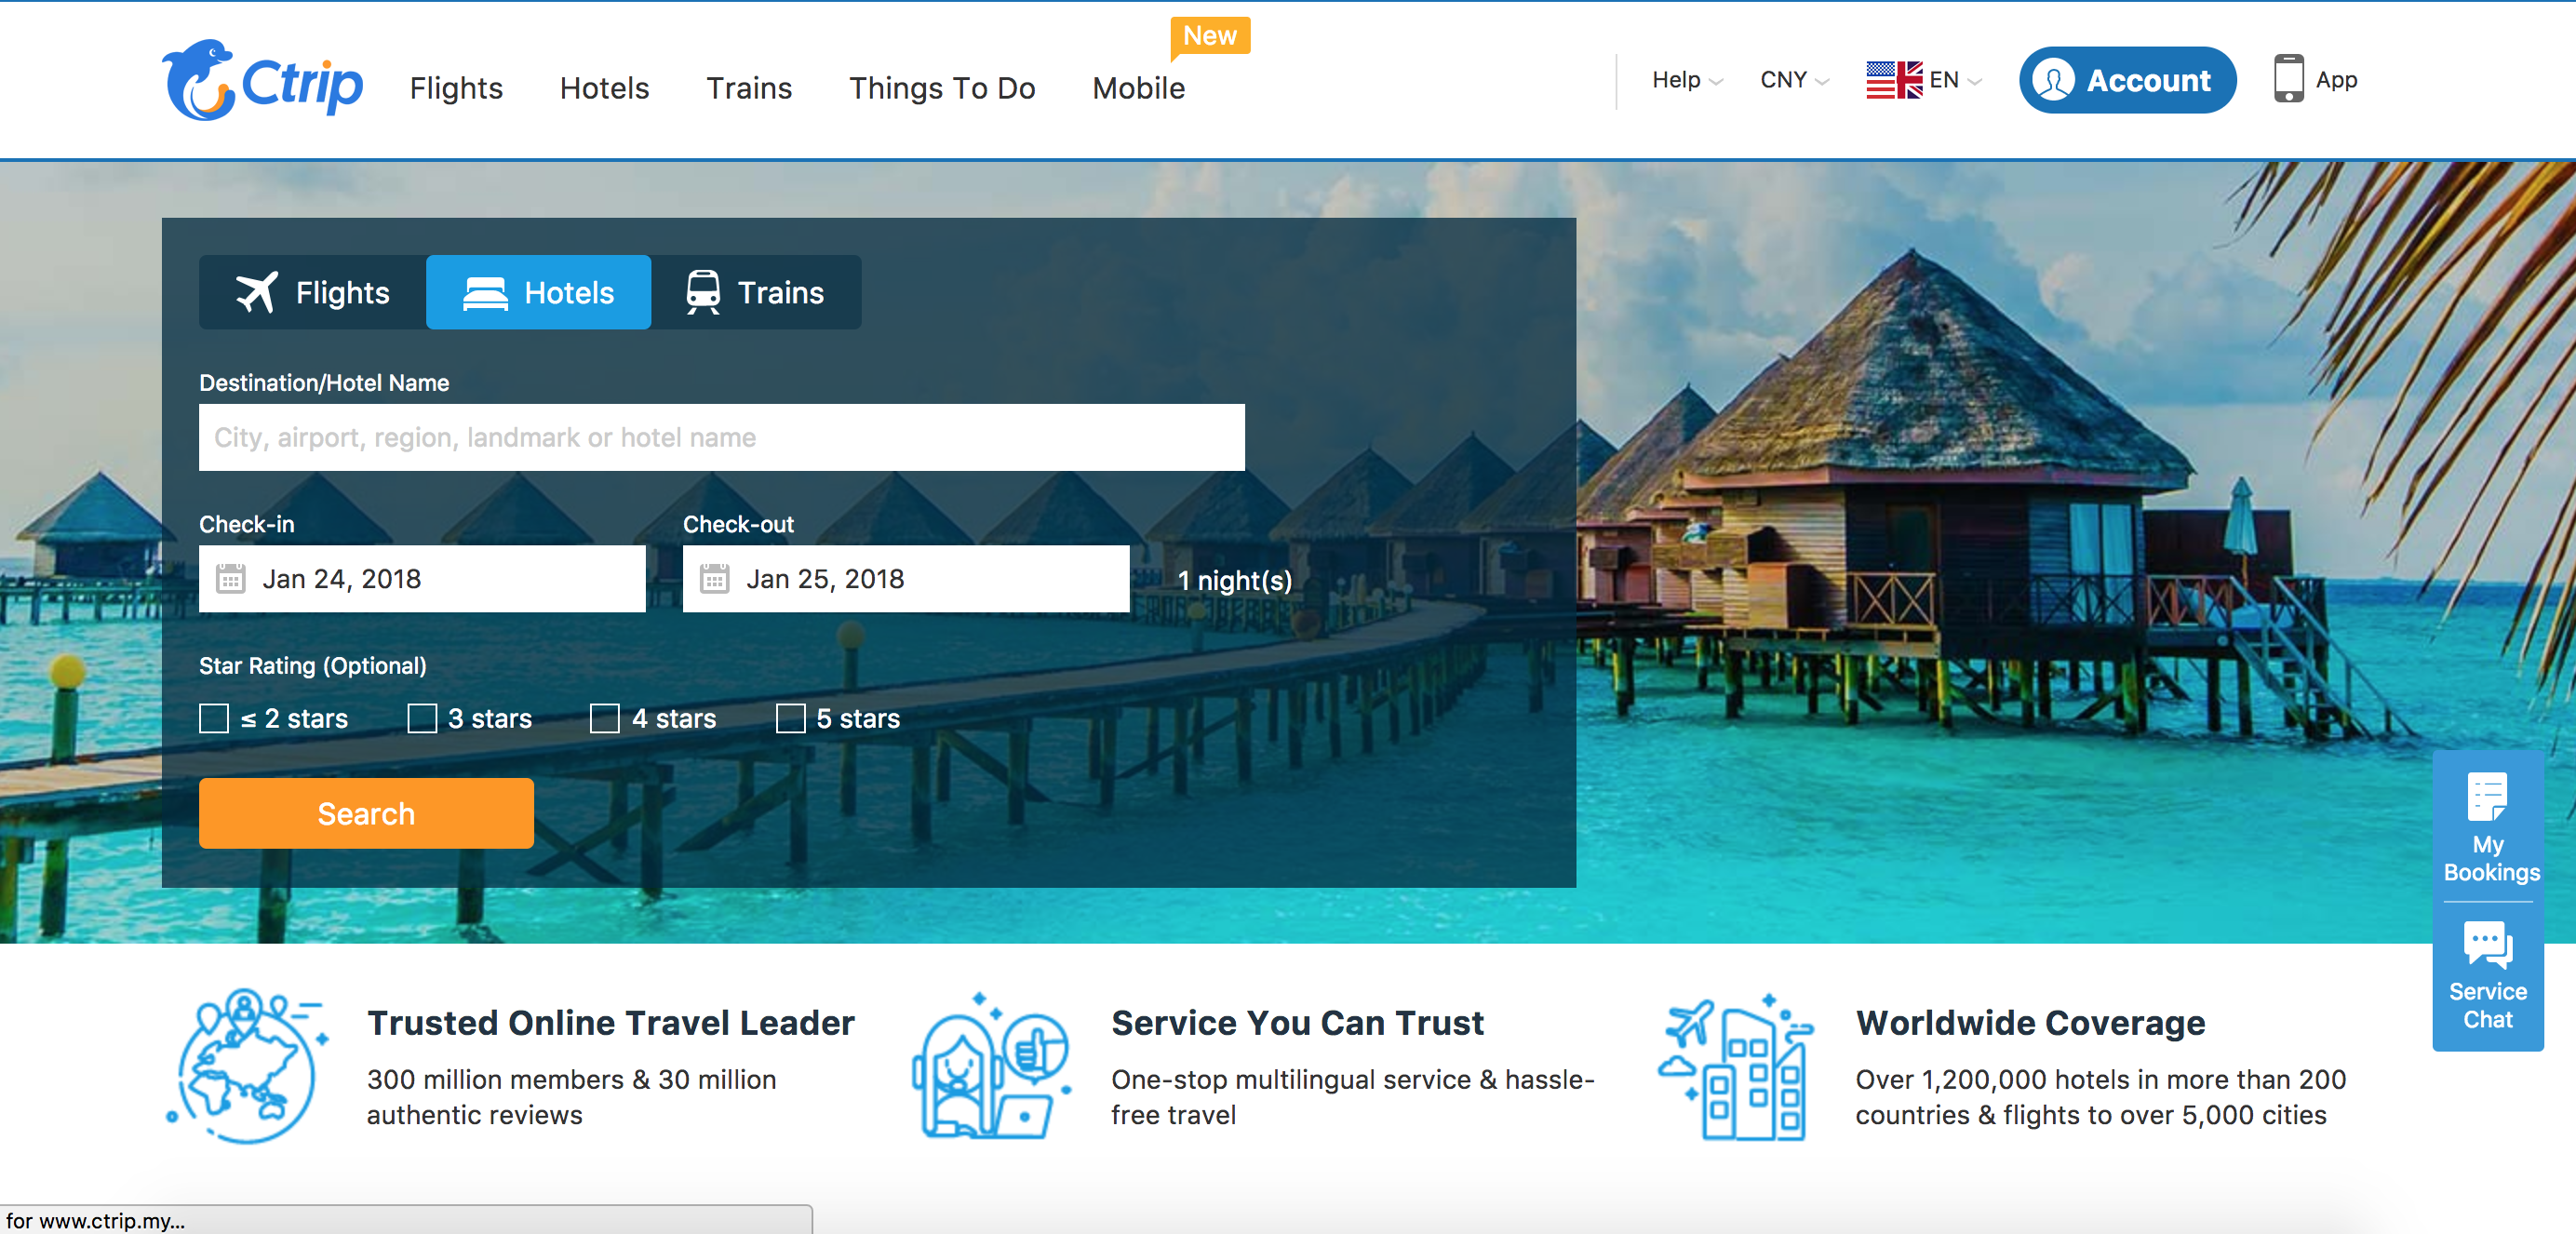
\includegraphics[width=100mm]{Images/ctrip_eng1}
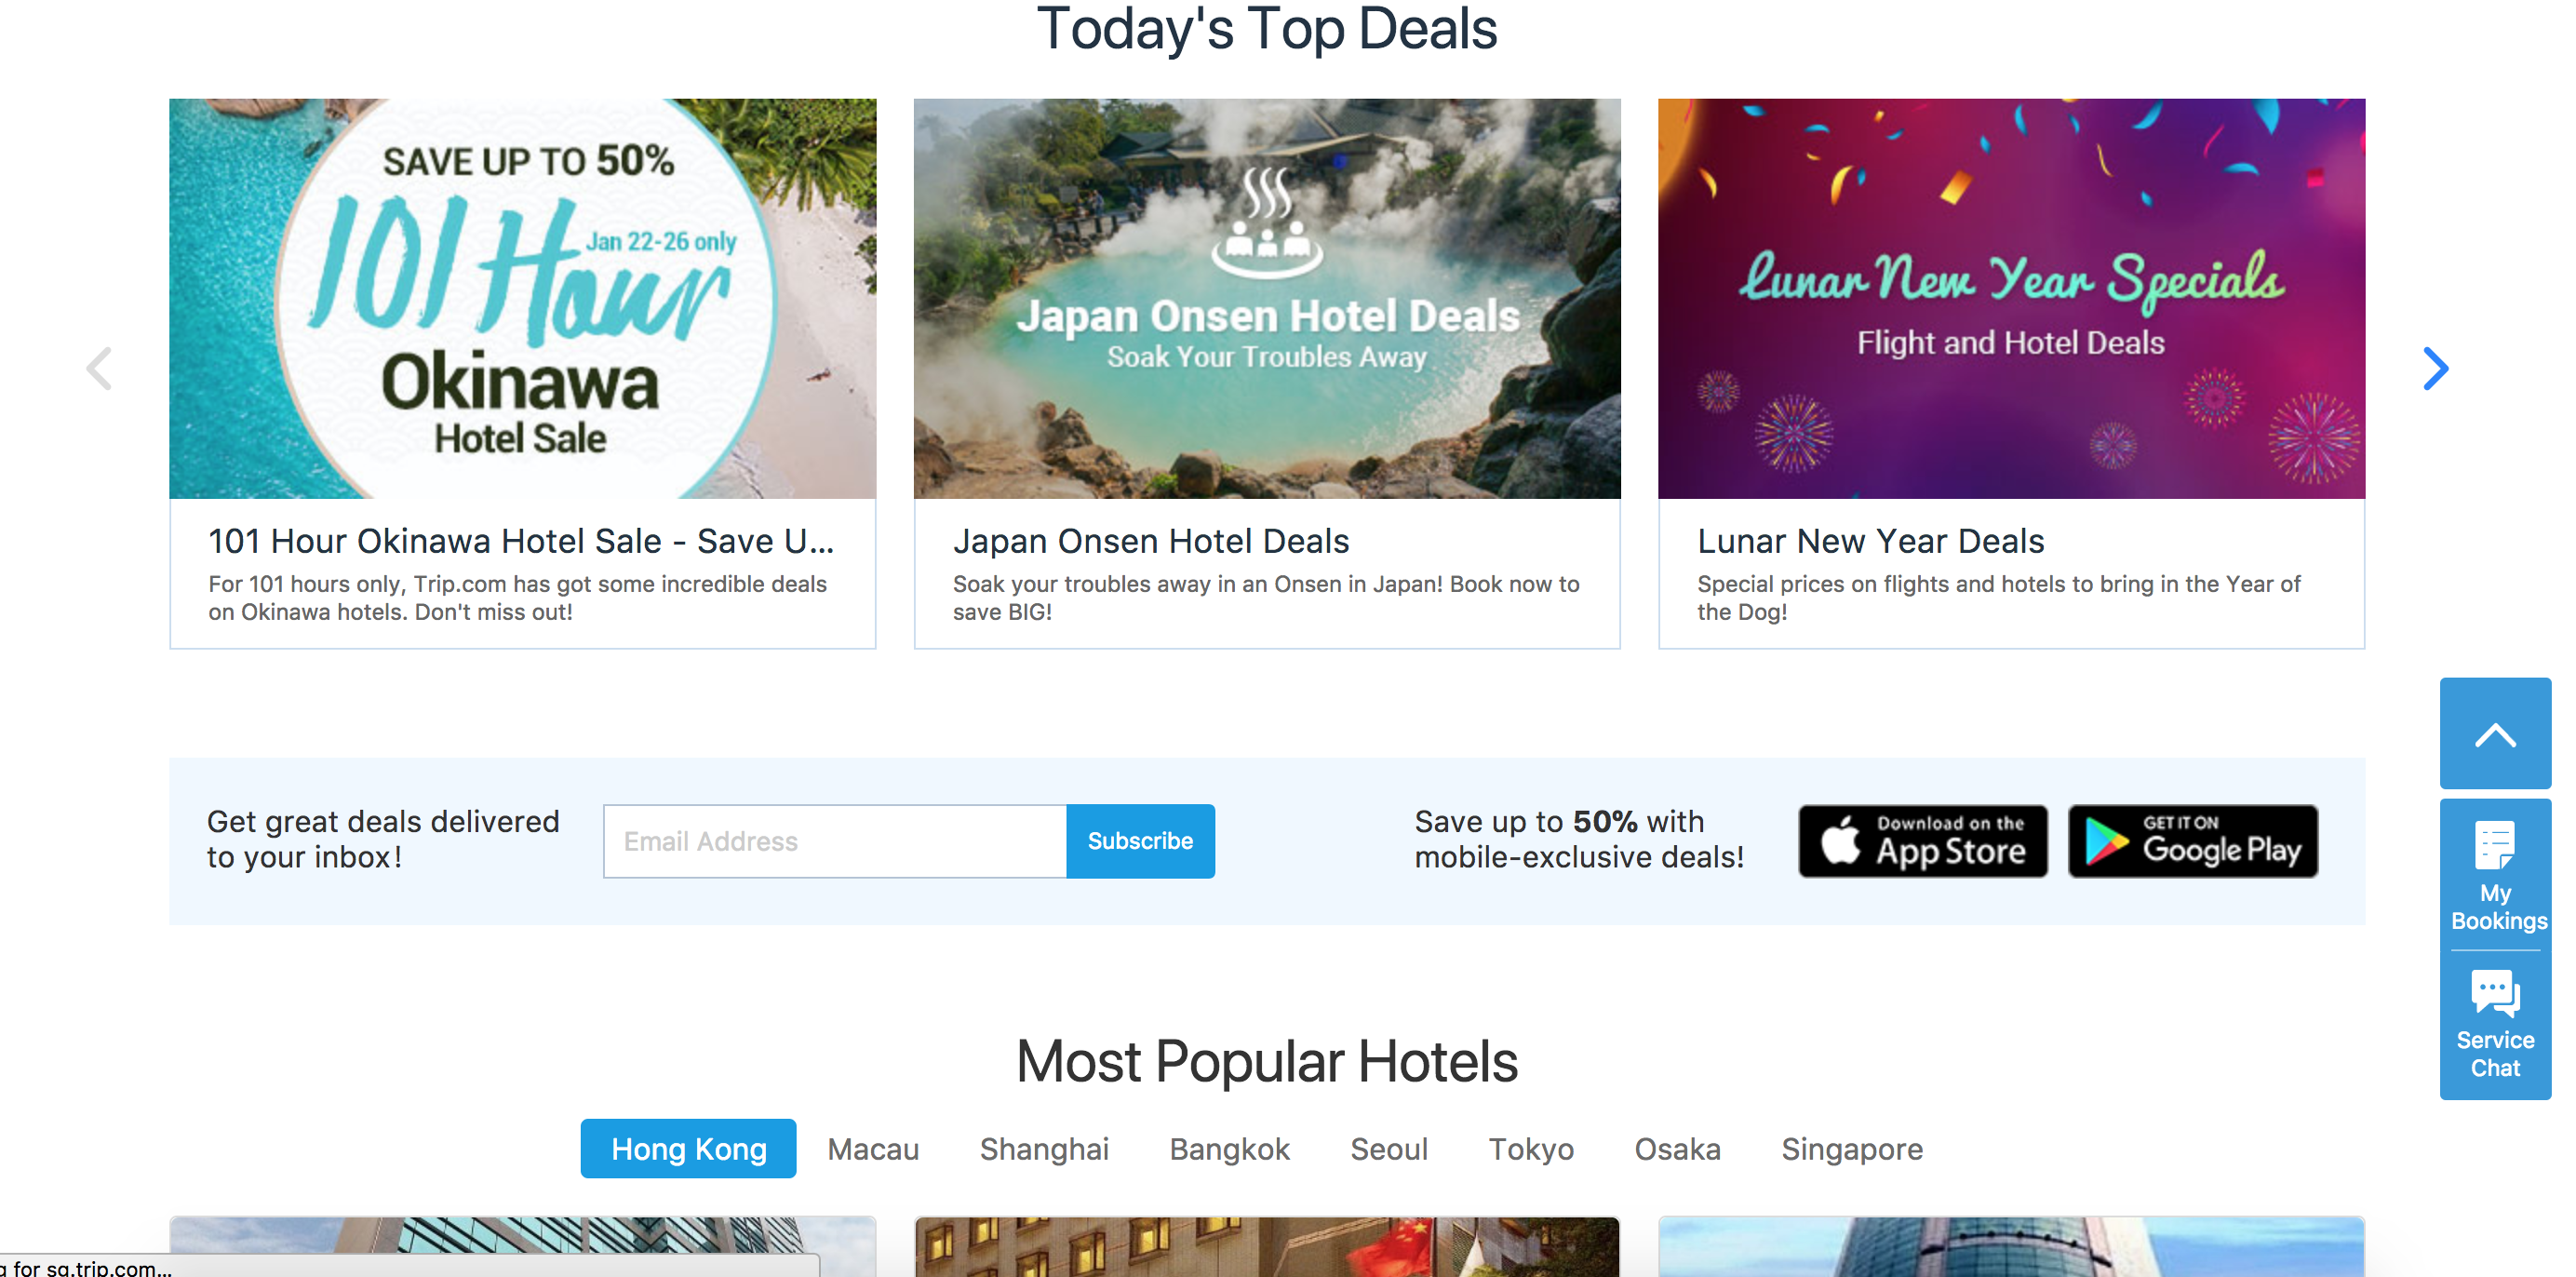
\includegraphics[width=100mm]{Images/ctrip_eng2}
\decoRule
\caption[English version of Ctrip]{The English version of the travel website Ctrip.}
\label{fig:ctrip_english}
\end{figure}
 The main difference we can see between these sites is the density of content. The Chinese version has a lot more content on a smaller area. Counting clickable elements without hovering over anything we can find 40 clickable elements on the Chinese version compared to 26 clickable elements on the English version. When using the Chinese site all links open a separate window instead of a second menu or tab. This is a quite common phenomena found in many sites.
 
 
 
\newpage
 \section{Conclusion Phase 1}
 \subsection{Common Chinese design that differs from western design}
Looking through the websites we can identify several design features (outside of the language differences) that differ in Chinese and western websites. 
\\\\
These are:
 \begin{itemize}
 \item High information density
 \item Colors
 \item Ad content
 \item Navigation
 \end{itemize}
 
 The main factor we could see across all websites is the difference in information density. Chinese websites have significantly higher information density compared to their western counterparts. This is one feature we want to examine more closely in our later study. Colors and navigation will be explored but not prioritized. These will be included to give a more accurate feel of the site instead of focused on. Chinese sites have a higher ad content than many of the western counterparts, this is a feature that not will be looked into in this study.   There are several hypothesis for why Chinese sites are so information dense. Some of these hypothesis are: cultural/trends, historical, holistic vs analytic perceptions (ref or cite..) and language. Because of limitations with understanding of the Chinese language, history and culture we will mainly examine trends and perception.
 \\\\
  To do this we will create two interfaces, one western inspired and one with inspiration from Chinese designs. To make sure that the interfaces will look Chinese and Western we will with the help from professional UX-designers from Sweden and China develop some prototypes. The prototypes will then be tested on both users with Swedish and Chinese heritage respectively. We will later develop a working interface from these prototypes that will be able to measure what the users do in response to certain tasks. Main measurements that will be used are task-success, time-on-task and System usability scale (cite???). 
 
 \subsection{Limitations}
 Even if many of the biggest websites in china are quite information dense there are several websites that have adopted a sleeker look for their sites/services. Two big examples of this is the messenger app WeChat which is very big in china and the the alipay service website. I will not focus on sites like this and there might be a trend in china that is moving towards a sleeker look. In this report i have specifically chosen the some of the most popular regularly used sites that differ from the western design standard. In the case of Taobao it might seem very difficult for many westerners to use but it is as of now one of the biggest websites in the world. There are also cases of websites more or less copying western websites because they are blocked in China. A typical example of this is youku and youtube, these types of sites will not be focused on in this report either.